% breadcrumb.tex - design document for the breadcrumb application

\documentclass{article}

\usepackage{graphicx}

\begin{document}

\title{Breadcrumb}
\date{\today}  %\today is replaced with the current date
\maketitle

\newpage
\tableofcontents
\newpage

\section{Aim}
Breadcrumb is an application which allows users to send text based messages across the internet.
The manner in which message transactions to occur will be such that:
\begin{itemize}
	\item \texttt{User Discovery} - Chat initialization occurs in a secure manner, immune to MITM attack
	\item \texttt{End-to-end encrypted} - Message plaintext is only available to the sender and intended recipient
	\item \texttt{Forward secrecy} - Key compromise does not allow previous messages to be decrypted
	\item \texttt{Internal Metadata Leaking} - User metadata is hidden from the Breadcrumb infrastructure
	\item \texttt{External Metadata Leaking} - User metadata is hidden from an adversary capable of observing network traffic
\end{itemize}

\section{Setup}
\subsection{OS Support}
\subsubsection{Client}
\begin{itemize}
	\item \texttt{GNU/Linux} - x86-64
\end{itemize}
\subsubsection{Node}
\begin{itemize}
	\item \texttt{GNU/Linux} - x86-64
	\item \texttt{GNU/Linux} - armhf
\end{itemize}
\subsection{Dependencies}
\begin{itemize}
	\item \texttt{OpenSSL} - https://www.openssl.org
	\item \texttt{miniupnpc} - http://miniupnp.tuxfamily.org/
\end{itemize}
\subsection{Getting Started}
\begin{enumerate}
	\item \texttt{Install OpenSSL}
		\begin{itemize}
			\item \texttt{Debian} - sudo apt-get install libssl-dev
			\item \texttt{From source} - https://www.openssl.org/source/
		\end{itemize}
	\item \texttt{Install Miniupnpnc}
		\begin{itemize}
			\item \texttt{Debian} - sudo apt-get install libminiupnpc-dev
			\item \texttt{From source} - http://miniupnp.tuxfamily.org/files/
		\end{itemize}
	\item \texttt{Clone Breadcrumb Repository}
		\begin{enumerate}
			\item git clone https://github.com/nyquist-prompt/breadcrumb
		\end{enumerate}
	\item \texttt{Building Client}
		\begin{enumerate}
			\item cd breadcrumb/client/
			\item make
		\end{enumerate}
	\item \texttt{Building Node}
		\begin{enumerate}
			\item cd breadcrumb/node/
			\item make
		\end{enumerate}
\end{enumerate}

\subsection{Running a Client}
\subsubsection{Compilation Switches}
The client compilation switches are located at the beginning of client.c and function as follows.
\begin{itemize}
	\item \texttt{ENABLE\_LOGGING} - Enable general logging
	\item \texttt{ENABLE\_TRANSMIT\_RECEIVE\_LOGGING} - Enable specific logging of transmit and receive events
	\item \texttt{ENABLE\_KEY\_HISTORY\_LOGGING} - Log all ephemeral breadcrumb keys
	\item \texttt{ENABLE\_BANDWIDTH\_LOGGING} - Log bandwidth to file (bandwidth.csv)
	\item \texttt{ENABLE\_TOTAL\_UID\_LOGGING} - Log all ephemeral breadcrumb uids (User IDs) to file
	\item \texttt{ENABLE\_UID\_HISTORY\_LOGGING} - Log all ephemeral breadcrumb uid history (User IDs) to file upon SIGINT
	\item \texttt{ENABLE\_USER\_INPUT\_THREAD\_LOGGING} - Enable specific logging of user input events
	\item \texttt{ENABLE\_PACKET\_DATA\_LOGGING} - Log all packet (transmit and recieve) data
	\item \texttt{ENABLE\_UID\_GENERATION\_LOGGING} - Log all generated ephemeral breadcrumb uids (User IDs)
	\item \texttt{LOG\_TO\_FILE\_INSTEAD\_OF\_STDOUT} - Redirect all logging to file (client\_$<$client name$>$.log)
	\item \texttt{LAN\_NETWORKING\_MODE} - Use LAN ip instead of WAN ip when NOT in test mode
	\item \texttt{TEST\_MODE} - Listen on ETH interface and connect to hard coded relays specified in function 'setup\_test\_mode\_conversation'
	\item \texttt{TEST\_MODE\_CLIENT\_1} - Define user as CLIENT 1 when in test mode, this hardwires the entry node
	\item \texttt{TEST\_RR\_PACKET} - Force send a 'return route' type packet
	\item \texttt{TEST\_UID\_CLASH} - Generate UIDs within a small range in order to test potential uid clashes
	\item \texttt{USING\_TEST\_HARNESS} - Client starts immediately (as opposed to waiting for '/connect' command)
\end{itemize}
\subsubsection{Starting a Client}
The start a client enter: ./client USER\_ID PORT
\subsubsection{Client Commands}
\begin{itemize}
	\item \texttt{/connect USER\_ID} - Initiate a chat with client with username USER\_ID
	\item \texttt{/network} - Perform network test (not implemented yet)
	\item \texttt{/exit} - Exit Breadcrumb
	\item \texttt{/leave} - Leave current conversation
	\item \texttt{/help} - Display command help
	\item \texttt{/testrr} - Force sending of a 'return route' type packet
\end{itemize}
\subsubsection{Test Mode}
Currently two clients may successfully communicate via the Breadcrumb infrastructure provided:
\begin{enumerate}
	\item Both clients have 'TEST\_MODE' enabled
	\item Only one client has 'TEST\_MODE\_CLIENT\_1' enabled
	\item Clients are connected to an ethernet switch
	\item Nodes, as defined in 'setup\_test\_mode\_conversation', are connected to the ethernet switch and executing
	\item Clients issue the '/connect' command, correctly specifying the other clients USER\_ID
\end{enumerate}
\subsection{Running a Node}
\subsubsection{Compilation Switches}
\begin{itemize}
	\item \texttt{ENABLE\_LOGGING} - Enable general logging
	\item \texttt{ENABLE\_LOG\_ON\_EXIT} - Log all relay data to file (relay\_log.csv) upon exit 
	\item \texttt{ENABLE\_THREAD\_LOGGING} - Log thread creation\/destruction events
	\item \texttt{ENABLE\_PACKET\_LOGGING} - Log all packet data
	\item \texttt{ENABLE\_UID\_LOGGING} - Log all received uid (user ID) data
	\item \texttt{LOG\_TO\_FILE\_INSTEAD\_OF\_STDOUT} - Redirect all logging to file ($<$relay name$>$.log)
	\item \texttt{SOFT\_RESET\_KEY\_STORE} - Upon startup do NOT regenerate key store
	\item \texttt{ENABLE\_BANDWIDTH\_REPORTING\_UI} - Client starts immediately (as opposed to waiting for '/connect' command)
\end{itemize}
\subsubsection{Starting a Node}
The start a node enter: ./node NODE\_ID PORT [LOGGING INTERVAL]
\subsubsection{Important}
When starting for the first time, a Node will create a keystore, which (depending upon the amount of free harddrive space) can be quite large. Thus it 
is advised to only start a Node on the intended machine - don't start one on your local machine 'just for fun'.

\newpage

\section{Concepts}
\subsection{Client}
A Client is a user who connects and performs message transactions with other users across the Breadcrumb infrastructure.
Clients are realized by executing the Breadcrumb client application on a users local machine (PC or mobile device) which is connected to the Internet.

\subsection{Node}
A Node hosts 'breadcrumbs' (UID + Ephemeral key) as well as user messages. Nodes use breadcrumbs (which are implanted by clients) in order to perform packet (onion-style) routing. User
messages are stored on the Node until it receives a matching 'return route' packet, which allows the Node to route the message to the intended recipient 
(see section 'Protocol' - 'Packet Routing'). Although Nodes perform only those two functions, with respect to a user conversation (which must use a finite set of Nodes) they
perform different tasks:
\begin{itemize}
	\item \texttt{Entry Node} - The only Node by which a client directly exchanges packets. All packets destined for other Nodes are onion-routed via this Node.
The Entry Node must be unique for all participants of a conversation.
	\item \texttt{Server Node} - A Node common to all conversation participants which is used to host user messages.
	\item \texttt{Relay Node} - A Node which may be common amongst participants and only used to relay packets destined for other Nodes.
\end{itemize}
Nodes are realized by untrusted third parties, primarily hosted on low-power/cost mini PCs (e.g. Raspberry Pi), which are connected to the Internet. 
Third parties who run Nodes are re-imbursed for their bandwidth expenditure (See 'Spider' and 'Economy' sections).

\subsection{Directory}
A Directory allows users to create a Breadcrumb IM account and provides users who wish to chat with a 'Chat Cookie'. It also connects to Nodes to enable the user chat (by enabling 
the storage of messages under that Conversation ID defined by that 'Chat Cookie'). The 'Chat Cookie' defines which Nodes are used by a particular user conversation (e.g. Entry Node, Server Node and Relay Nodes) and are
selected based on the current amount of clients using a particular Node with respect to that Nodes maximum capacity (which varies depending upon its specific hardware). Thus
Directories ensure that the total traffic passing amongst the Node Network does not exceeded its capability and also that it is evenly spread.
Directories are realized by trusted third parties.

\subsection{Spider}
A Spider is a single client which simply passes traffic throughout the Node Network in order to ascertain Node uptime. The uptime is recorded and used to correctly re-imburse
Nodes for their bandwidth. Spiders also ensure a minimum amount of traffic is passing through the Node Network to ensure adequate packet mixing (which obscures packet metadata)
is occuring.

\newpage

\section{Networking}
\subsection{Figures}
The figures used in the following section are described as follows:

\begin{figure}[h]
\centering
\begin{minipage}{.3\textwidth}
  	\centering
  	
\includegraphics[width=1.7cm,height=1.7cm,keepaspectratio]{img/Directory.png}
	\caption{Directory}
\end{minipage}
\begin{minipage}{.3\textwidth}
  	\centering
	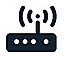
\includegraphics[width=1.5cm,height=1.5cm,keepaspectratio]{img/Node.png}
	\caption{Node}
\end{minipage}
\begin{minipage}{.3\textwidth}
  	\centering
	
\includegraphics[width=1.4cm,height=1.4cm,keepaspectratio]{img/Client.png}
	\caption{Client}
\end{minipage}
\end{figure}

\subsection{Client Registration}
Clients register with a single Directory (Figure 4), encrypting the transfer via HTTPS as well as the Directories 2048-bit RSA key (which is packaged as part of the client application).
The registration request is routed via TOR to ensure that the Directory cannot equate a request with an IP address. The Directory then accepts or rejects the registration, 
depending upon the existence of a client ID clash. Client ID and password is hashed (SHA-2) prior to transfer. If a registration is approved it is synchronized amongst the other 
Directories (Figure 5).
\begin{figure}[h]
\centering
\begin{minipage}{.4\textwidth}
  	\centering
  	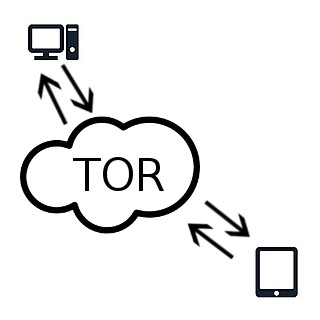
\includegraphics[width=4cm,height=4cm,keepaspectratio]{img/ClientRegistration.png}
	\caption{Client Registration}
\end{minipage}
\begin{minipage}{.4\textwidth}
  	\centering
	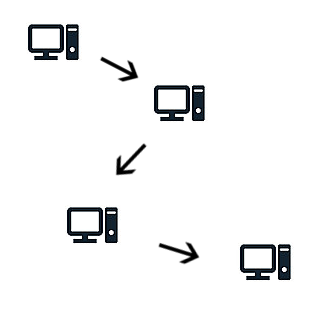
\includegraphics[width=4cm,height=4cm,keepaspectratio]{img/RegistrationSync.png}
	\caption{Registration Sync}
\end{minipage}
\end{figure}

\subsection{Chat Initialization}
Chat initialization occurs similarly to Client Registration. A Client that wishes to begin a conversation with another client first contacts the Directory server (via TOR), providing the hashed
username of the other member of the conversation. The Directory server creates a 'Chat Cookie' and attempts to synchronize it amongst the other Directories. In the case that another
Directory already has a cookie with the same conversation ID (i.e. the other member of the conversation initialized the chat first) the cookie with the more recent timestamp is discarded
and the older cookie is returned to the Client that made the request. The Directory then registers the conversation ID with the conversation Server Node as per Figure 6.
\begin{figure}[h]
  	\centering
  	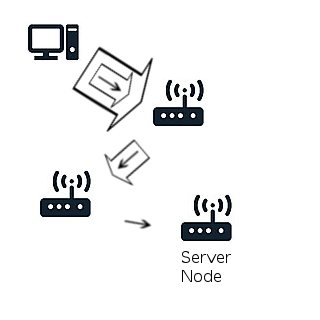
\includegraphics[width=4cm,height=4cm,keepaspectratio]{img/MessageIDRegistration.png}
	\caption{Enabling conversation in Server Node}
\end{figure}


\subsection{Routing}
In order to route packets via the Node Network, a Client must first implant 'breadcrumbs' (see section 'Protocol' - 'Breadcrumb'). As per the protocol, Clients may only
inject packets into the Node Network via the Entry Node; implanting breadcrumbs is no exception. If a Client wishes to implant breadcrumbs with a non-Entry Node, it 
must onion route the implant packet via the Entry node as per Figure 7. In order to mask the metadata from an external observer the implant of breadcrumbs must be performed 
via an encrypted channel. In order to maximize performance, a Client uses DH Eliptical Curve to encrypt the breadcrumb implant packet. Once an initial set of breadcrumbs is 
implanted, subsequent packets that retrieve that breadcrumb will leave new breadcrumbs in their wake. Thus a breadcrumb is completely ephemeral - after it is retrieved it is 
discarded by the Node and replaced with the breadcrumb that is defined in the packet that triggered its retrieval.
\begin{figure}[h]
\centering
\begin{minipage}{.4\textwidth}
  	\centering
  	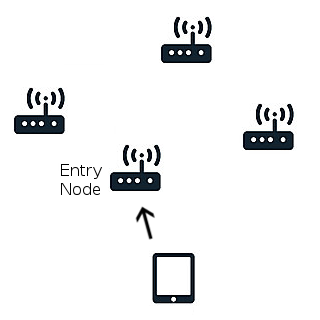
\includegraphics[width=4cm,height=4cm,keepaspectratio]{img/BreadcrumbPlacement.png}
	\caption{Implanting breadcrumbs with an Entry Node}
\end{minipage}
\hspace{1cm}
\begin{minipage}{.4\textwidth}
  	\centering
	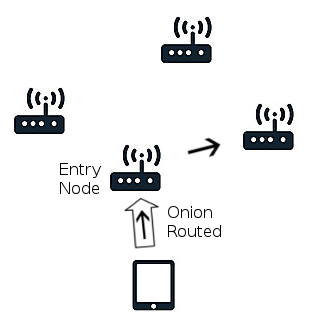
\includegraphics[width=4cm,height=4cm,keepaspectratio]{img/BreadcrumbPlacement1.png}
	\caption{Implanting breadcrumbs with a non-Entry Node}
\end{minipage}
\end{figure}

\newpage

\subsection{Sending Messages}
A client transmits a message by sending a Message Packet. A Message Packet consists of text that is to be transferred to the receiving client wrapped 
in an onion route made up of a random non-Entry Node as the first hop and the recieving clients' Entry Node as the second hop. The conversation ID and 
hash of the Node IDs that make up the route to the receiving client is appended to the packet. This allows the the Server Node to match the message packet 
to a particular conversation and pair it with a Return Route Packet (see below) which is provided by the receiving client. This is then wrapped in an onion 
route that consists of the clients Entry Node, a random non-Entry Node and finally the Server Node and transmitted (Figure 9).
\begin{figure}[h]
	\centering
  	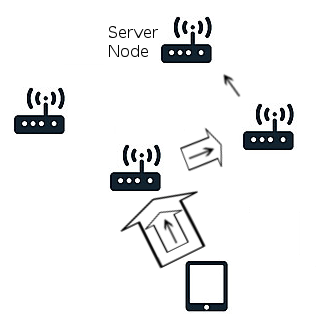
\includegraphics[width=6cm,height=6cm,keepaspectratio]{img/MessagePacket.png}
	\caption{Routing a Message Packet to the Server Node}
\end{figure}

\subsection{Receiving Messages}
A return route packet defines an onion route that is capable of being paired to a message packet and the entirety is transmitted back to the client that provided it.
A client that wishes to receive a message generates an onion route that consists of a random non-Entry Node as the first hop and its Entry Node as the second. The
Node IDs of this route are hashed and appended to allow the Server Node to pair it with a message packet. This is then wrapped in an onion route that consists of the clients Entry Node,
a random non-Entry Node and finally the Server Node and transmitted (Figure 10).
\begin{figure}[h]
	\centering
  	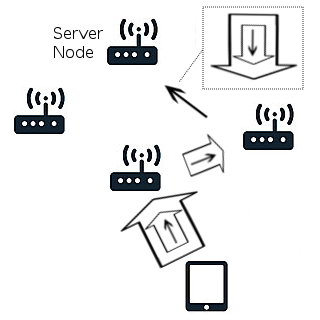
\includegraphics[width=6cm,height=6cm,keepaspectratio]{img/ReturnRoutePacket.png}
	\caption{Routing a Return Route Packet to the Server Node}
\end{figure}

\subsection{Constant Bandwidth}
Dummy packets are primarily used by a client to ensure a constant bandwidth in the case that there are no message packets to create and all possible return route
packets have been defined and transmitted. They also serve to obscure the identity of the Server Node which in turn furthers the obscurity of the other conversation participant.
Dummy packets may be singular in direction (Figure 11) and are discarded by the final Node defined in their onion route, or may define a return onion route and are
eventually transmitted back to the client. In the latter case they serve to obscure the timing of conversation messages (as they are indistinguishable from the perspective
of an external observer) and are also used by the Client to test the Node Network. For example, a Client can ascertain if a Node has gone offline through logical deduction
based on the route it defined and whether or not it received a dummy packet.
\begin{figure}[h]
	\centering
  	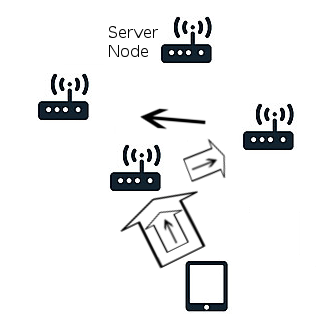
\includegraphics[width=6cm,height=6cm,keepaspectratio]{img/DummyPacket.png}
	\caption{Routing a non-Return Route style Dummy Packet}
\end{figure}

\newpage

\section{Data Structures}

\subsection{Breadcrumbs}
The datastructure that enables onion routing, a 'breadcrumb', is defined as such:\\*\\*
\texttt{\-\hspace{1cm}typedef struct breadcrumb\\*
\-\hspace{1cm}\{\\*
\-\hspace{2cm}uint8\_t key[AES\_KEY\_SIZE\_BYTES];\\*
\-\hspace{2cm}uint32\_t uid;\\*
\-\hspace{1cm}\} breadcrumb;\\*\\*}
Where AES\_KEY\_SIZE\_BYTES = 16 (128-bit AES). The breadcrumb UID is used as an index for key storage and retrieval by a Node. UID clashes are currently resolved by
using a linked-list at a particular UID index. For example, if a Node receives a packet with UID = X it first attempts to decrypt the current onion layer by applying
AES key at index X. If that fails (determined via the veracity of the decrypted checksum value) the Node moves to the next key in the linked-list and again attempts
to decrypt the packet. If the packet decryption is successful the key is removed and the new UID / key pair is added to the key storage (see 'Packet Structure' - 'Onion Route Data' section).

\subsection{Packet Structure}
The core datastructure of Breadcrumb is the packet structure (see Figure 12 - following page). The beginning of the 'Route Onion 1' section is a valid breadcrumb UID (that was registered previously),
transmitted in plaintext, which is used by the Node to find the corresponding breadcrumb key and decrypt the rest of the 'Route Onion' section. The same applies to the 'Payload Onion' section. The specifics of the individual 'Onion Route' and 'Payload Onion' are also defined on the following page. Note the 'Next IP' and 'Next Port' fields are simply filled with random data in the case that the packet section is 'Payload Onion'.
\newpage
\texttt{\-\hspace{0.5cm}typedef struct onion\_route\_data\\*
\-\hspace{1cm}\{\\*
\-\hspace{2cm}uint8\_t iv[AES\_KEY\_SIZE\_BYTES];\\*
\-\hspace{2cm}uint32\_t uid;\\*
\-\hspace{2cm}uint32\_t align\_filler1;\\*
\-\hspace{2cm}uint64\_t align\_filler2;\\*
\-\hspace{2cm}onion\_route\_data\_encrypted ord\_enc;\\*
\-\hspace{1cm}\} onion\_route\_data;\\*\\*
\-\hspace{1cm}typedef struct onion\_route\_data\_encrypted\\*
\-\hspace{1cm}\{\\*
\-\hspace{2cm}uint64\_t next\_pkg\_ip;\\*
\-\hspace{2cm}uint16\_t next\_pkg\_port;\\*
\-\hspace{2cm}uint16\_t ord\_checksum;\\*
\-\hspace{2cm}uint32\_t new\_uid;\-\hspace{3.5cm}// Next breadcrumb UID\\*
\-\hspace{2cm}uint8\_t new\_key[AES\_KEY\_SIZE\_BYTES]; // Next breadcrumb key\\*
\-\hspace{1cm}\} onion\_route\_data\_encrypted;\\*}
\begin{figure}[h]
	\centering
  	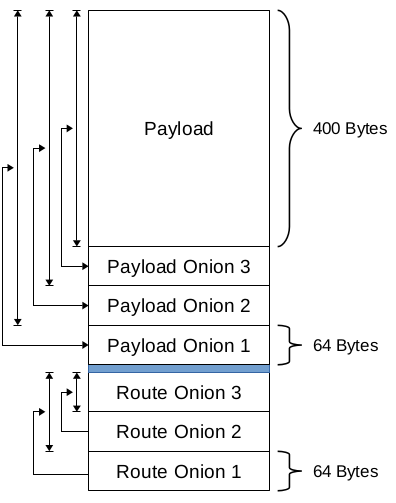
\includegraphics[width=8cm,height=8cm,keepaspectratio]{img/BasicPacketStructure.png}
	\caption{Packet Structure}
\end{figure}

\newpage

\subsection{Packet Types}
There are four packet types, which are described in the following sections. The packet type, as defined in the packet metadata, is included in the 'Payload' of the Breadcrumb Packet. The generic structure of the payload is defined as follows:\\*\\*
\texttt{\-\hspace{1cm}typedef struct payload\_data\\*
\-\hspace{1cm}\{\\*
\-\hspace{2cm}uint16\_t type;\\*
\-\hspace{2cm}uint16\_t onion\_r1;\\*
\-\hspace{2cm}uint16\_t onion\_r2;\\*
\-\hspace{2cm}uint16\_t order;\\*
\-\hspace{2cm}uint32\_t client\_id;\\*
\-\hspace{2cm}uint32\_t conversation\_id;\\*
\-\hspace{2cm}uint8\_t payload[PAYLOAD\_SIZE\_BYTES];\\*
\-\hspace{1cm}\} payload\_data;}\\*\\*
The fields of the packet metadata are as follows:
\begin{itemize}
	\item \texttt{type} - Enumeration defining the packet type.
	\item \texttt{onion\_r1} - If type is 'Dummy Packet /w Return Route' then this is the port for the transmitted packet. If type is 'Message Packet' then this is the XOR of the relay IDs (return route) and conversation ID. If
	type is 'Return Route' this is the XOR of the relay IDs (return route) and conversation ID of the first defined return route.
	\item \texttt{onion\_r2} - If type is 'Return Route' this is the XOR of the relay IDs (return route) and conversation ID of the second defined return route. Otherwise it is unused (random data).
	\item \texttt{order} - If the type is 'Message Packet' this is the conversation packet order otherwise it is unused (random data).
	\item \texttt{client\_id} - The client ID of the packet sender unless the packet is 'Dummy Packet /w Return Route' in which it is the most significant two bytes of the IP address for the transmitted packet.
	\item \texttt{conversation\_id} - If the type is 'Message Packet' or 'Return Route' this is the conversation ID. If the packet is 'Dummy Packet /w Return Route' in which it is the least significant two bytes of the IP address for the transmitted packet.
\end{itemize}

\subsubsection{Dummy Packet}
A dummy packet is essentially the same as Figure 12 (previous pages), except the 'Payload' is simply random data.
\newpage
\subsubsection{Dummy Packet /w Return Route}
A dummy packet /w return route is a packet that defines a return route within the 'Payload' section.\\*\\*
\begin{figure}[h]
	\centering
  	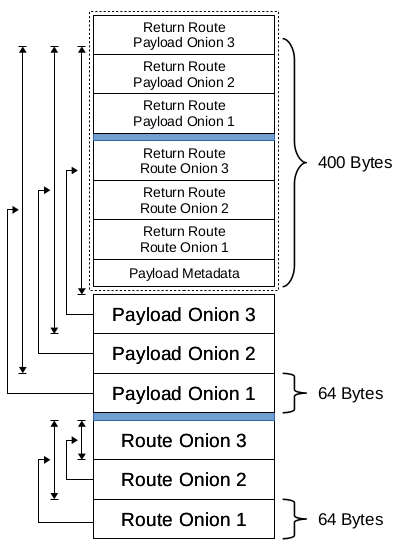
\includegraphics[width=8cm,height=8cm,keepaspectratio]{img/DummyPacketWReturnRoute.png}
	\caption{Dummy Packet /w Return Route}
\end{figure}
\newpage
\subsubsection{Message Packet}
A message packet contains a message destined for the other conversation participant within its 'Payload' section. The message itself is wrapped in a onion return route that is comprised of a random non-entry node followed by the entry node (both with respect to the user receiving the message).\\*\\*
\begin{figure}[h]
	\centering
  	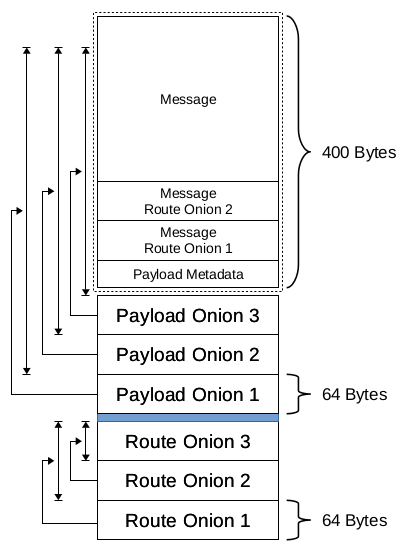
\includegraphics[width=8cm,height=8cm,keepaspectratio]{img/MessagePacketStructure.png}
	\caption{Message Packet}
\end{figure}
\newpage
\subsubsection{Return Route Packet}
A return route packet contains two onion routes that are capable of being paired to a message packet (transmitted by the other conversation participant) to form a packet that may be transmitted back to the client that provided the
return route packet. The packet metadata fields, onion\_r1 and onion\_r2, are the XOR of the relay IDs (and conversation ID) that make up the onion route that is defined. The fields, 'Return Route ID 1' and 'Return Route ID 2' are made up of random data which is cached by the Client that sends the Return Route Packet. In the event that a Client receives a Message Packet, it is these fields that are used to determine which return route the packet took. This is required in order to determine which breadcrumb (key / uid) pairs are now present in the return route Nodes.\\*\\*
\begin{figure}[h]
	\centering
  	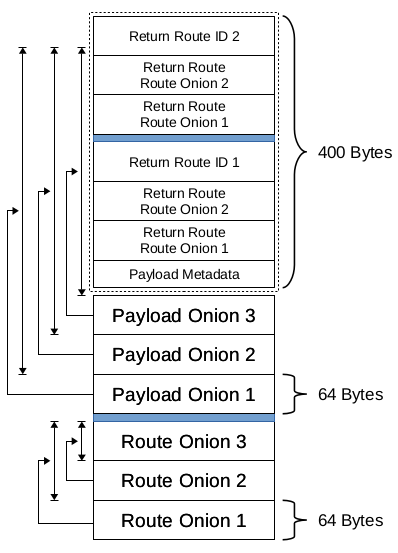
\includegraphics[width=8cm,height=8cm,keepaspectratio]{img/ReturnRoutePacketStructure.png}
	\caption{Return Route Packet}
\end{figure}
\newpage

\section{Processes}
\subsection{Enabling Routes}
Directores enable routes by pushing cookie to Node (part of Chat Cookie). Nodes confirm packet was sent by Directory by checking against list of hard-coded key signatures.
\subsection{Enabling Message Exchange}
Directory enables message exchange by pushing cookie to Node in particular Message Slot. Nodes confirm packet was sent by Directory by checking against list of hard-coded key signatures.
\subsection{Routing Packets}
As described in section 'Packet Structure' after receiving a packet the Node decrypts the 'Route Onion' and 'Payload Onion' sections. After decryption, the 'Next IP' address of the 'Route Onion' section is compared with '0.0.0.0',
if equal it is a 'Non-routing Packet', otherwise it is a 'Routing' packet. The packet is thus reconfigured as Figure 16, the filler being random data that is appended to preserve the constant packet size and then sent to the 'Next IP'.
\begin{figure}[h]
	\centering
  	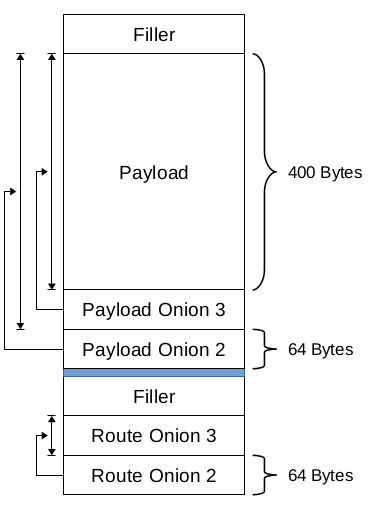
\includegraphics[width=8cm,height=8cm,keepaspectratio]{img/BasicPacketStructurePostRoute.png}
	\caption{Post Routing Packet}
\end{figure}
\newpage
\subsection{Non-routing Packets}
The manner in which non-routing packets are handled is dependent upon the packet-type, as 
\begin{itemize}
	\item \texttt{Dummy Packet} - Nodes simply discard Dummy Packets upon receiving them.
	\item \texttt{Dummy Packet /w Return Route} - Upon receiving a Dummy Packet /w Return Route a node discards the payload metadata and positions the return route data (onion and payload) at the beginning of the packet. The Node then pads the packet with random data such that it is the standard packet size and then transmits the packet.
	\item \texttt{Message Packet} - Upon receiving a Message Packet a Node will cache the packet if the message slot (determined by the conversation ID and user ID as set by the 'Message') has been enabled by a Directory and is currently empty, otherwise the Message Packet is discarded.
	\item \texttt{Return Route} - Upon receiving a Return Route packet a Node checks both 'onion IDs' against the onion ID of any messages in the message slot (determined by the conversation ID). If a match is found, the corresponding return route (first for onion\_r1, second for onion\_r2) is coupled with the message and the packet is transmitted. Otherwise the return route packet is simply discarded.
\end{itemize}

\subsection{Forward Secrecy}
Before message transaction occurs, clients will perform a DH key exchange and derive a session key. This session key will be used (as well as the Chat Cookie session key) as the root key of an Axolotl ratchet. \cite{OwsRatchet,AxoRatchetLib} Clients will identify DH key exchange packets by the return route that they occur upon - the 'Chat Cookie' will define a specific, unique return route path that will be used by clients to ONLY transmit DH packets.

\newpage

\section{Scalability}
The maximum number of Breadcrumb users is entirely dependent upon the number of Nodes in the Node Network. As a client is only able to use the Node Network after successfully obtaining a 'Chat Cookie' from a Directory, Directories will 'throttle' the number of clients such that it remains within the maximum (and the maximum for each individual Node). Message latency will be only slightly affected by the number of clients using the Node Network as the set of Nodes that are used as part of a conversation is only a small set of the total Nodes, i.e. messages do not transverse all Nodes, only a small subset.
The number of clients an individual Node can accommodate will be dependent upon:
\begin{itemize}
	\item \texttt{Memory} - The amount of available RAM determines the size of the key store (i.e. number of breadcrumbs a Node can accommodate) and message store.
	\item \texttt{Performance} - The rate at which the client can perform cryptographic bottlenecks (DH Elliptical Curve).
	\item \texttt{Bandwidth} - The total bandwidth and RX/TX rate.
\end{itemize}

\section{Economy}
TODO (Nodes are reimbursed for uptime)

\newpage

\section{Attack Vectors}
\subsection{Malicious Nodes}
As Nodes are run by Untrusted Third Parties they could potentially be malicious and logging/analyzing network traffic. Since traffic is end-to-end encrypted this type of attack could never result in the attacker recovering conversation plaintext, however it could result in the unmasking of conversation participants. However, in order to do so, the malicious actor would have to control the Server Node, as well as both Entry Nodes and one non-Entry node used by participant A and one non-Entry node used by participant B. If any of the aforementioned requirements are not fufilled, either one or both of the conversation participants are obscured. Both scenarios are detailed as follows (red represents malicious Nodes):\\*\\*
\begin{figure}[h]
	\centering
  	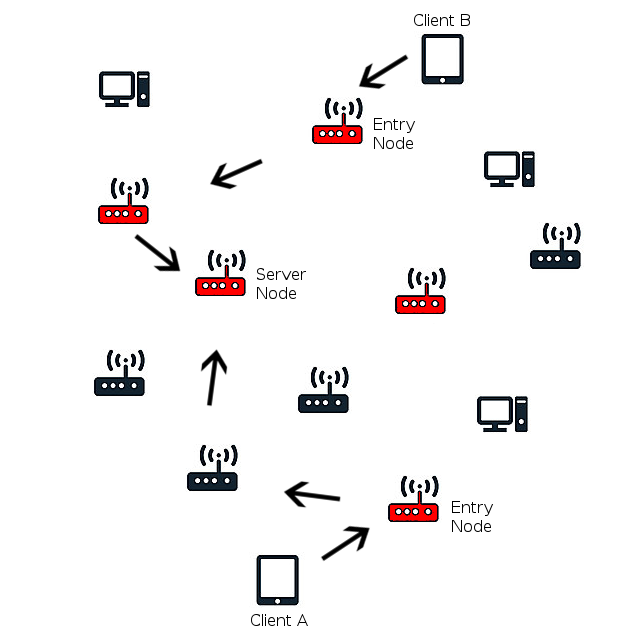
\includegraphics[width=8cm,height=8cm,keepaspectratio]{img/UnCompromisedConversation.png}
	\caption{Uncompromised Conversation}
\end{figure}
\begin{figure}[h]
	\centering
  	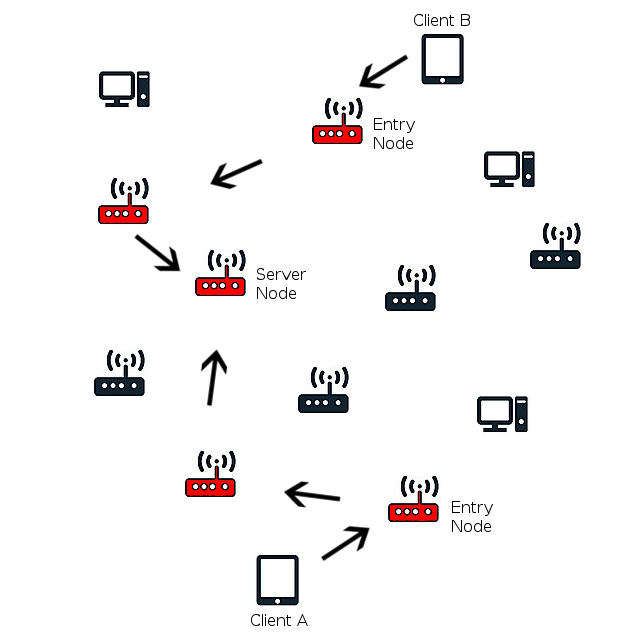
\includegraphics[width=8cm,height=8cm,keepaspectratio]{img/CompromisedConversation.png}
	\caption{Compromised Conversation}
\end{figure}

\newpage

\subsection{DDOS}
TODO (DDOSing the Node Network)

\section{Future Work}
Potential improvements include:
\begin{itemize}
	\item \texttt{Pure Hardware Node} - Convert Nodes to be FPGA based (e.g. pure hardware). Improves security (no potential for operating system flaw exploit), performance and reduces cost, physical size and power consumption.
\end{itemize}

\newpage

\begin{thebibliography}{9}
	\bibitem{OwsRatchet} Open Whisper Systems, \emph{Advanced cryptographic ratcheting}. https://whispersystems.org/blog/advanced-ratcheting/, 26 Nov 2013.
	\bibitem{AxoRatchetLib} Axolotl, \emph{ Axolotl C Library}. https://github.com/WhisperSystems/libaxolotl-c, 23 Dec 2015.

\end{thebibliography}

\end{document}